\chapter{Wavelets and Gabor Filters}
\label{ch:lesson16}

The Fourier transform (Chapter~\ref{ch:lesson15}) tells you \emph{which} frequencies are present in a signal, but not \emph{where} --- a sine wave basis function extends across the entire image, so a localized feature (an edge, a texture patch) gets smeared across the whole spectrum. \textbf{Wavelets} and \textbf{Gabor filters} are two different fixes for this: both are built from small, spatially localized oscillations instead of infinite sinusoids, giving a joint sense of \emph{where} and \emph{what frequency}.

\section{The Haar wavelet: the simplest possible wavelet}

The Haar wavelet transform splits a signal into an \textbf{approximation} (local averages) and a \textbf{detail} (local differences), computed on non-overlapping pairs of samples:
\begin{equation}
a_k = \frac{x_{2k} + x_{2k+1}}{\sqrt{2}}, \qquad d_k = \frac{x_{2k} - x_{2k+1}}{\sqrt{2}}.
\end{equation}
This should look familiar: it's essentially the same ``blur $+$ keep the residual'' idea as the Laplacian pyramid (Chapter~\ref{ch:lesson13}), just computed pairwise instead of with a Gaussian kernel, and without overlap between neighborhoods. A manual NumPy computation matches \code{pywt.dwt(signal, 'haar')} exactly.

\section{From Haar to Daubechies: smoother wavelets}

The Haar wavelet is discontinuous (a hard step), which gives it poor frequency localization --- its own frequency content is spread out, the opposite of what we want. \textbf{Daubechies wavelets} (\citelink{daubechies1988}{Daubechies, 1988}) use longer, smoother filters with more \emph{vanishing moments}, trading a wider spatial support for much better frequency behavior. \code{db2} (sometimes called ``D4'' for its 4 filter taps) is the next step up in smoothness from Haar, shown in Figure~\ref{fig:l16-1}.

\begin{figure}[h]
\centering
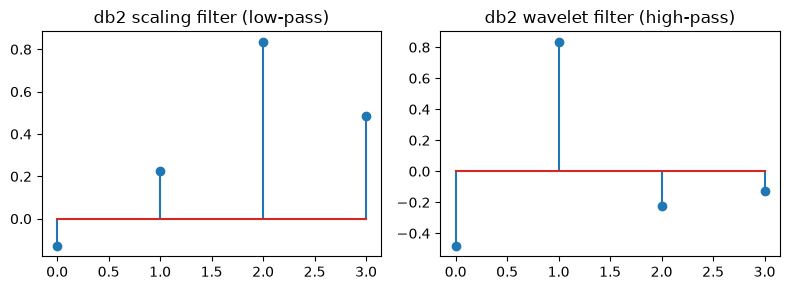
\includegraphics[width=0.75\textwidth]{figures/lesson16_fig01.png}
\caption{\code{db2}'s scaling (low-pass) and wavelet (high-pass) filters, four taps each.}
\label{fig:l16-1}
\end{figure}

The Haar transform above is just a convolve-and-downsample-by-2 operation with the 2-tap filters $[\tfrac{1}{\sqrt2},\tfrac{1}{\sqrt2}]$ and $[\tfrac{1}{\sqrt2},-\tfrac{1}{\sqrt2}]$. Daubechies wavelets follow the exact same recipe with longer filters. A from-scratch periodic-convolution implementation of \code{db2}'s decomposition matches \code{pywt} exactly, and inverting it (\code{pywt.idwt}) reconstructs the original signal perfectly.

\section{2D wavelet decomposition of an image}

Like the separable Gaussian filter in Chapter~\ref{ch:lesson10}, a 2D wavelet transform is applied as two 1D passes: rows, then columns. One level of decomposition splits an image into \textbf{four subbands}:
\begin{itemize}
  \item \textbf{LL}: low-pass both directions --- a coarser, half-resolution copy of the image (like one Gaussian pyramid level)
  \item \textbf{LH}: low-pass rows, high-pass columns --- responds to horizontal edges
  \item \textbf{HL}: high-pass rows, low-pass columns --- responds to vertical edges
  \item \textbf{HH}: high-pass both directions --- responds to diagonal detail and corners
\end{itemize}
Figure~\ref{fig:l16-2} shows all four subbands for a test image.

\begin{figure}[h]
\centering
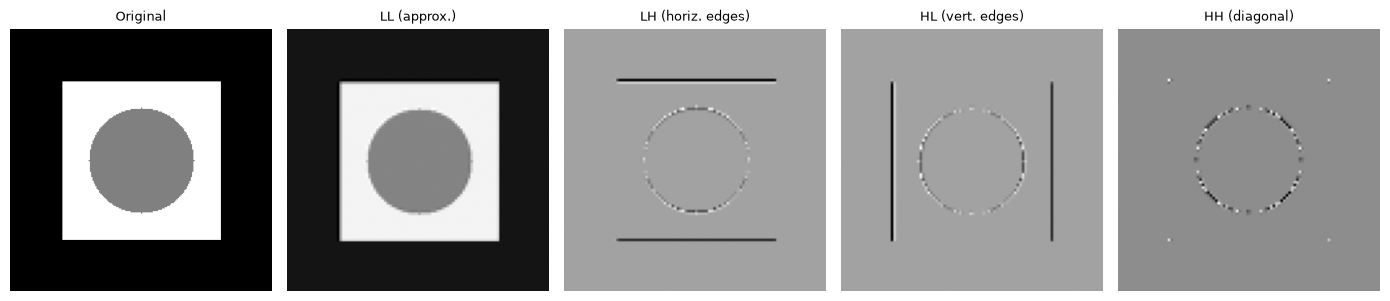
\includegraphics[width=0.95\textwidth]{figures/lesson16_fig02.png}
\caption{A test image and its four \code{db2} subbands.}
\label{fig:l16-2}
\end{figure}

Just like the Laplacian pyramid, this decomposition is exactly invertible: \code{pywt.idwt2} reconstructs the original from the four subbands with essentially no loss (max error $1.4\times10^{-13}$, floating-point roundoff).

\section{Gabor filters: localized oscillations tuned to orientation}

A \textbf{Gabor filter} is a sinusoidal grating multiplied by a Gaussian envelope --- a wave that's localized in space, tuned to a specific frequency \emph{and} orientation. Unlike Daubechies wavelets (built for compact, orthogonal, invertible multi-resolution decomposition), Gabor filters are used more for \emph{feature extraction}: detecting oriented texture and edges at a chosen scale.

Gabor filters also have a striking biological connection. Recording neurons in a cat's visual cortex, Hubel and Wiesel (\citelink{hubelwiesel1959}{Hubel \& Wiesel, 1959}) found ``simple cells'' that fire selectively for a bar or edge at one specific orientation and position, and barely at all for other orientations --- a foundational discovery in visual neuroscience. It was later shown (\citelink{marcelja1980}{Marcelja, 1980}; \citelink{daugman1985}{Daugman, 1985}) that a 2D Gabor function is a remarkably good mathematical model of these simple-cell receptive fields, part of why Gabor filters became a standard, biologically-motivated tool for orientation-selective feature extraction in computer vision. Figure~\ref{fig:l16-3} shows a bank of Gabor kernels across several orientations and wavelengths.

\begin{figure}[h]
\centering
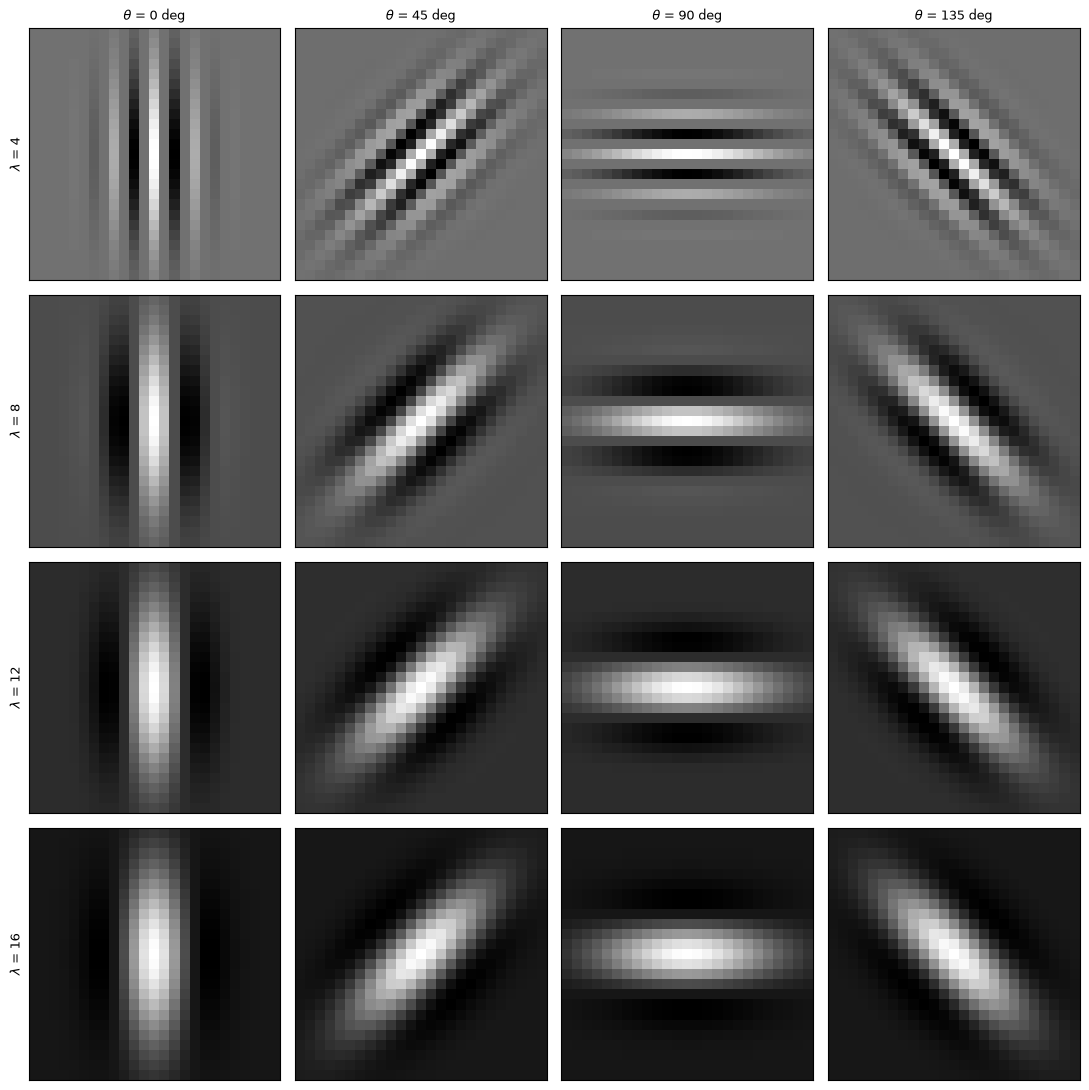
\includegraphics[width=0.6\textwidth]{figures/lesson16_fig03.png}
\caption{Gabor kernels across four orientations ($\theta$) and four wavelengths ($\lambda$).}
\label{fig:l16-3}
\end{figure}

\subsection*{Orientation selectivity, demonstrated quantitatively}

Four bars at four different orientations (Figure~\ref{fig:l16-4}), each filtered with a Gabor kernel tuned to each orientation; a filter should respond most strongly to the bar matching its tuning and weakly to the others.

\begin{figure}[h]
\centering
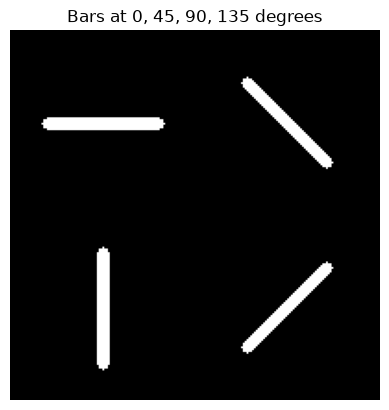
\includegraphics[width=0.35\textwidth]{figures/lesson16_fig04.png}
\caption{Test bars at $0^\circ$, $45^\circ$, $90^\circ$, $135^\circ$.}
\label{fig:l16-4}
\end{figure}

\begin{center}
\renewcommand{\arraystretch}{1.3}
\begin{tabular}{lrrrr}
\hline
\textbf{Filter tuned for} & \multicolumn{4}{c}{\textbf{Response to bar at}} \\
 & $0^\circ$ & $45^\circ$ & $90^\circ$ & $135^\circ$ \\
\hline
$0^\circ$   & \textbf{2580} & 612 & 343 & 612 \\
$45^\circ$  & 495 & \textbf{3277} & 495 & 428 \\
$90^\circ$  & 343 & 612 & \textbf{2580} & 612 \\
$135^\circ$ & 495 & 428 & 495 & \textbf{3277} \\
\hline
\end{tabular}
\end{center}

The response matrix is strongly diagonal-dominant: each filter's largest response (bold) lands squarely on the bar it was tuned for, exactly the orientation selectivity Hubel and Wiesel observed biologically.

\subsection*{Exercises}
\begin{enumerate}
  \item Try \code{db4} (\code{pywt.Wavelet('db4')}) instead of \code{db2} for the 2D image decomposition. How does the LH/HL/HH subband appearance change, given \code{db4}'s longer, smoother filters?
  \item Apply \code{pywt.dwt2} a second time to the LL subband from the image decomposition above, to get a second, coarser level --- this is a \textbf{wavelet pyramid}, directly analogous to the Gaussian/Laplacian pyramids of Chapters~\ref{ch:lesson11} and \ref{ch:lesson13}.
  \item Increase \code{lambd} (the sinusoid's wavelength) in the Gabor kernel while keeping \code{sigma} fixed. What happens to the number of visible stripes inside the Gaussian envelope, and how would you expect that to change which real-image texture scale the filter responds to?
\end{enumerate}

\vfill
\fullcode{lesson16}{lesson16_wavelets_gabor}
